\documentclass[tikz,border=8pt]{standalone}
\usepackage{fontspec}
\setsansfont{Arial}
\usetikzlibrary{arrows.meta,positioning}
\begin{document}
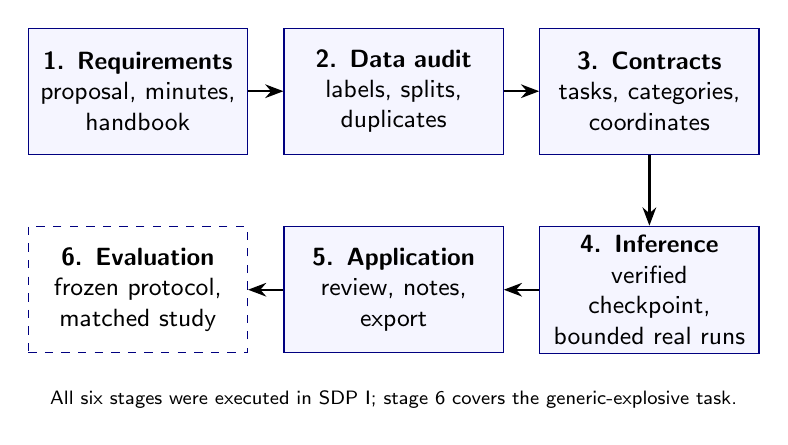
\begin{tikzpicture}[font=\sffamily\small,>=Stealth,
box/.style={draw=blue!50!black,align=center,text width=2.55cm,minimum height=1.6cm,fill=blue!4},
plan/.style={box,dashed,fill=white}]
% Stages of the engineering method used in SDP I (Section 1.1.3).
\node[box] (s1) {\textbf{1. Requirements}\\proposal, minutes,\\handbook};
\node[box,right=0.45cm of s1] (s2) {\textbf{2. Data audit}\\labels, splits,\\duplicates};
\node[box,right=0.45cm of s2] (s3) {\textbf{3. Contracts}\\tasks, categories,\\coordinates};
\node[box,below=0.9cm of s3] (s4) {\textbf{4. Inference}\\verified checkpoint,\\bounded real runs};
\node[box,left=0.45cm of s4] (s5) {\textbf{5. Application}\\review, notes,\\export};
\node[plan,left=0.45cm of s5] (s6) {\textbf{6. Evaluation}\\frozen protocol,\\matched study};
\draw[->,thick] (s1)--(s2);\draw[->,thick] (s2)--(s3);\draw[->,thick] (s3)--(s4);
\draw[->,thick] (s4)--(s5);\draw[->,thick] (s5)--(s6);
\node[below=0.35cm of s5,align=center,font=\sffamily\scriptsize] {All six stages were executed in SDP I; stage 6 covers the generic-explosive task.};
\end{tikzpicture}
\end{document}
